\lecture{16}{17 aprile 2024}
\section{Pressione di radiazione}
Come le onde meccaniche, anche le onde elettromagnetiche trasportano energia (\(\langle u_{EM} \neq 0 \rangle \)). Associato alle onde elettromagnetiche c'è anche il vettore di Poynting, che ha valore medio diverso da zero (quindi trasporta qualcosa!). Si può mostrare che il vettore di Poynting è in grado di esercitare una pressione "di radiazione" sui corpi. Trasportano anche momento angolare, ma questo lo scopriremo in meccanica quantistica.
Ma come nasce la pressione di radiazione? Studiamo il comportamento di una carica positiva (\(q>0\)) in un mezzo conduttivo in presenza di un'onda elettromagnetica di questo tipo:
\begin{align}
	\vec{E}(z,t)&= E_0 \cos (kz- \omega t) \vec{\hat{i}} & 
	\vec{B}(z,t)&=\frac{E_0}{v} \cos (kz - \omega t) \vec{\hat{j}}
\end{align}
\begin{figure}[H]
	\begin{minipage}[t]{0.5\textwidth}
        \centering
        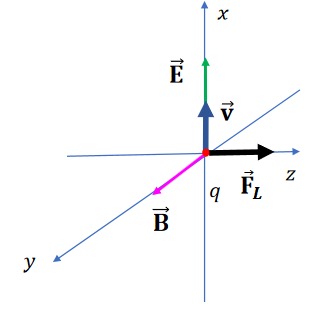
\includegraphics[width=0.6\linewidth]{screenshots/2024-04-18-09-25-40.png}
    \end{minipage}%
	\hfill%
    \begin{minipage}[t]{0.5\textwidth}
        \centering
        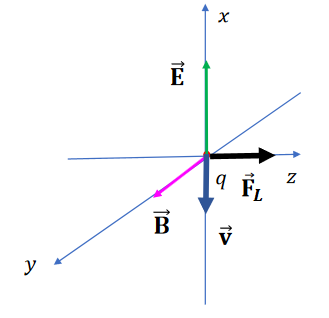
\includegraphics[width=0.6\linewidth]{screenshots/2024-04-18-09-34-09.png}
    \end{minipage}
\end{figure}
Il campo elettrico mette in moto la carica e, essendo in un mezzo conduttivo dove vale \(\vec{E}=\rho _R \vec{J}=\rho _R n q \vec{v}\), otteniamo che \(\vec{v} \propto \vec{E}\). Avendo una velocità verso le x positive, la carica subisce una forza di Lorentz diretta lungo l'asse z positivo per tutta la fase dell'onda in cui la componente del campo elettrico è positiva. Quando il campo elettrico si ribalta (quindi anche la velocità della carica) e va verso il basso, anche il campo magnetico inverte il suo verso e quindi il risultato netto è che la forza di Lorentz è diretta anche in questo caso nel verso di propagazione. Nel caso di una carica negativa non cambia nulla! Complessivamente la forza di Lorentz dipende da \(q ^{2} \), quindi ha sempre lo stesso verso indipendentemente dal segno della carica.

Consideriamo ora una piastra metallica con superficie \(\Sigma \) e \(N\) cariche libere sulla superficie. Su ogni carica agisce una forza data da \(\vec{F}=q \vec{E} + q \vec{v} \cp \vec{B}\), quindi sull'intera piastra si avrà una forza complessiva pari a \(\vec{F}_{tot} = Nq (\vec{E}+ \vec{v} \cp \vec{B})\). La forza elettrica oscilla e quindi mediamente è nulla, ma quella di natura magnetica ha sempre la stessa direzione. La potenza media fornita dall'onda alla piastra è data da
\begin{equation}
	\langle \mathcal{P} \rangle = \langle \vec{F}_{tot} \cdot \vec{v} \rangle = \langle N q \vec{E} \cdot \vec{v} \rangle 
\end{equation}
che ci dà la potenza spesa per unità di area:
\begin{equation}
	\left\langle \frac{\mathcal{P} }{\Sigma } \right\rangle =
	\left\langle \frac{Nq \vec{E}\cdot \vec{v}}{\Sigma } \right\rangle 
	= \sigma \langle \vec{E}\cdot \vec{v} \rangle 
\end{equation}
Se l'onda elettromagnetica viene completamente assorbita dalla piastra, si ha che la potenza spesa per unità di area è uguale all'intensità dell'onda iniziale:
\begin{equation}
	I = \left\langle \frac{\mathcal{P} }{\Sigma } \right\rangle 
	= \sigma \langle \vec{E}\cdot \vec{v} \rangle 
\end{equation}

Abbiamo visto che la forza di Lorentz è diretta sempre nella direzione di propagazione dell'onda. Per onde elettromagnetiche che si incontrano quotidianamente le oscillazioni sono molto rapide, il campo magnetico ha modulo \(\vert \vec{B} \vert = \quotient{\vert \vec{E} \vert }{c}  \) e le velocità massime degli elettroni sono significativamente inferiori a quelle della luce. Quindi la forza elettrica è sempre dominante rispetto a quella di Lorentz e si può approssimare la direzione di \(\vec{v}\) con quella di \(\vec{E}\), ottenendo quindi:
\begin{equation}
	\langle \vec{F}_{tot} = N \langle \vert q\vec{v} \cp \vec{B} \vert  \rangle  \rangle 
	= \frac{Nq \langle \vec{v} \cdot \vec{E}  \rangle }{c}
\end{equation}
Da questo si trova che la pressione è
\begin{equation}
	p = \left\langle \frac{\vec{F}_{tot} }{\Sigma } \right\rangle =
	\frac{\sigma }{c} \langle \vec{E} \cdot \vec{v} \rangle =
	\frac{I}{c}=
	\frac{\langle \vert \vec{S} \vert  \rangle }{c}
\end{equation}

\paragraph{Nota storica} Misurare la pressione di radiazione è molto difficile perché è necessaria un'intensità molto alta! I primi radiometri dell''800 funzionavano al contrario, perché l'effetto dell'onda era di scaldare una delle due facce della piastra metallica e quindi le molecole di gas spingevano leggermente la piastra avendo velocità leggermente diverse da un lato della piastra e dall'altro. Oggi la pressione di radiazione è utilizzata per i viaggi spaziali con le vele solari.